%!TEX root = ../thesis.tex
% Spellcheck ignore
% cSpell:ignore freerunning, detuning, microresonator, misestimates, Mathematica, modelfit, kappaplot, isat, powermeter, mathrm, giga, kappamodelratio, realrubidium, hyperfine, kappacorrection, intcorrection, powercorrection, multicolumn, extracolsep, toprule, midrule, bottomrule, fitplot, gaussians, nonumber, spectrumlegend, FWHM, diaminplot, meanplot, diaplot, bigskip, captionof, minipage, pagebreak, wincam, includegraphics,wrapfigure, ifpdf, graphicspath
%*******************************************************************************
%****************************** Fourth Chapter *********************************
%*******************************************************************************
\chapter{Evaluation}

% **************************** Define Graphics Path **************************
\ifpdf{}
    \graphicspath{{Chapter4/Figs/Raster/}{Chapter4/Figs/PDF/}{Chapter4/Figs/}}
\else
    \graphicspath{{Chapter4/Figs/Vector/}{Chapter4/Figs/}}
\fi

The scanning span we used was more than the \SI{6.86}{\giga\hertz} of the hyperfine
splitting of \(^{87}\)Rb. We thus observe four absorption dips due to \(^{87}\)Rb 
\(F=1\) and \(F=2\) and \(^{85}\)Rb \(F=2\) and \(F=3\). In the data analysis,
we treated each of the dips as a two-level atom, using the theory described in
Chapter 2.\\
We are interested in determining \(I_{s}\), which is included in \(\kappa'_0 \)
(see Eq.~\ref{eq:kappa_final}). We will use the Beer-Lambert law 
\( I(x)=I_0~\mathrm{e}^{-\kappa x} \), which leads on resonance to
\begin{align}
    I(x,\nu_0) = I_0~\mathrm{e}^{-\kappa'_0 x}~.
\end{align}
Which gives us an expression for \(\kappa'_0\)
\begin{align}\label{eq:kappa_prime}
    \kappa'_0 = -\frac{1}{L}~\ln\left(\frac{I(L,\nu_0)}{I_0} \right)
\end{align}
where \(L\) is the cell length. \\
Thus, one needs to extract from the absorption spectroscopy dips \(I(L,\nu_0) \)
and \(I_0\). We measured \(I(L,\nu_0,I_0) \) for different values of \(I_0\) and 
computed the experimental \(\kappa_0\). We will then fit the theory formula
~\ref{eq:kappa_final} using \(I_{s}\) and \(T\) as free parameters to extract 
them for the four ``atoms''. 

\pagebreak
%********************************** % First Section  **************************************
\section{Model fit on absorption spectra}~\label{sec:modelfit} %Section - 4.1
\begin{figure}[H]
    \centering
    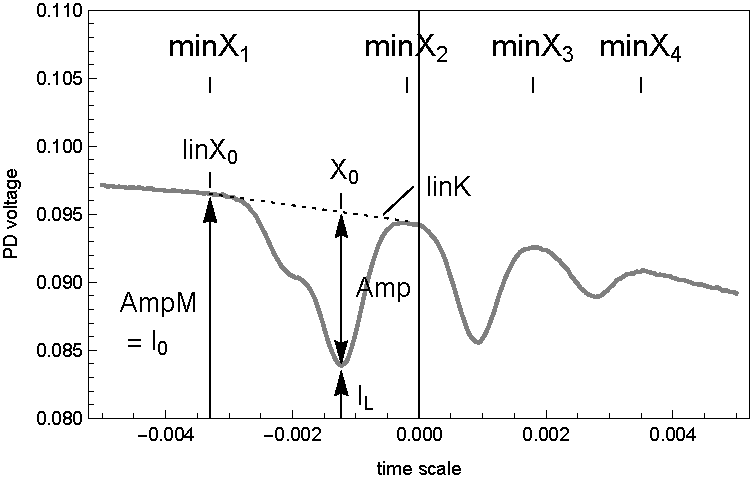
\includegraphics[width=.6\textwidth]{spectrumlegend}
    \caption{\label{fig:spectrumlegend} Definition of all model parameters for the
    \(^{85}\)Rb \(F=3\) line.}
\end{figure}

The whole data analysis and parameter fitting has been made using mathematica.
To narrow down the range for our fits of the different lines we defined four
constants \(minX_1\) to \(minX_4\) which mark the beginning or the end of one dip. 
As can be seen in Equation~\ref{eq:kappa_final} all our spectra are based on a 
gaussian model, but due to the short separation of the \(^{87}\)Rb \(F=2\) and 
\(^{85}\)Rb \(F=3\) line we have also an overlapping double gaussian. To reduce 
mode hopping the laser adjusted the beam power during the scan and therefore our 
spectra have a linear decrease in power. Our fitting models are based on a double 
and two single gaussians. For the explanation of all the parameters we will use 
the \(^{85}\)Rb \(F=3\) line as an example (see Fig.~\ref{fig:spectrumlegend}).
\begin{align}
    Gauss1 &= AmpM-Amp\cdot Exp\left(-\frac{{(x-x_0)}^2}{2~\sigma^2} \right) +
                linK(x-linX_0)  \\
    Gauss2 &= AmpM-Amp1\cdot Exp\left(-\frac{{(x-x_1)}^2}{2~{\sigma_1}^2} \right)-
                  Amp2\cdot Exp\left(-\frac{{(x-x_2)}^2}{2~{\sigma_2}^2} \right) \nonumber \\
                  &+ linK(x-linX_0)~,
\end{align}
where \(AmpM\) is the maximum power without absorption, \(Amp\) is the amplitude 
of the absorption, \(x_0\) is the center of the absorption line, \(\sigma \) is 
the standard deviation of the gaussian, \(linK\) is the slope of the power 
decrease and \(linX_0\) is the beginning of the gaussian. In case of the double 
gaussian the different parameters of the gaussians are labeled with the indices 
``1'' and ``2''.\\
With these two models all the spectra where fitted and the obtained parameters 
where saved into a single table for further analysis. The error bars of the
fits where saved into a separate table, which we will use for the uncertainties
of the absorption coefficient. One example of the fitted models is shown 
in Fig.~\ref{fig:fitplot}. All the info we want is contained in \(AmpM\) and \(Amp\).
\begin{figure}[H]
    \centering
    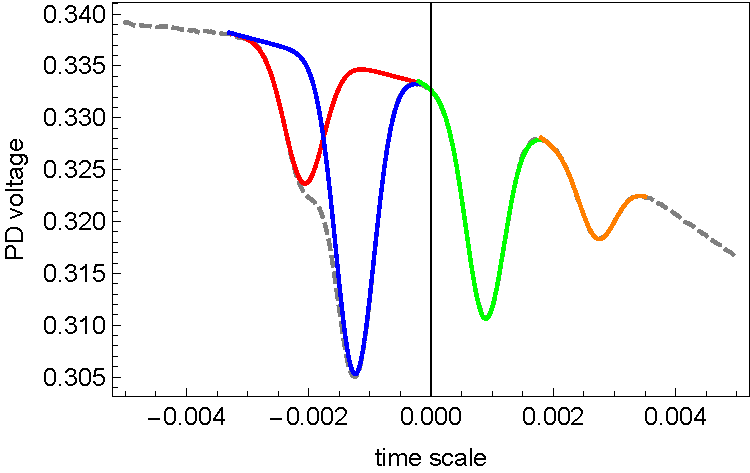
\includegraphics[width=.8\textwidth]{fitplot}
    \caption{\label{fig:fitplot} Absorption spectrum at \SI{350}{\micro\watt}
    with the fitted absorption lines.}
\end{figure}

\pagebreak
%********************************** % Second Section  **************************************
\section{Power extraction} %Section - 4.2

To link \(AmpM\) to the power measured with the powermeter, we need to take into
account that the power measured before the cell corresponds to the mean value
over the scanning range. For that reason we calculated the power at each transition 
position, assuming a linear decline and considering that the mean value lies in 
the middle of the minimum and maximum power (see Fig.~\ref{fig:powercorrection}). 
We applied these corrections for all our data sets. An example of the extracted 
powers can be found in Table.~\ref{table:powercorrection}. The error bars come 
from the powermeter uncertainties.

\begin{figure}[H]
    \centering
    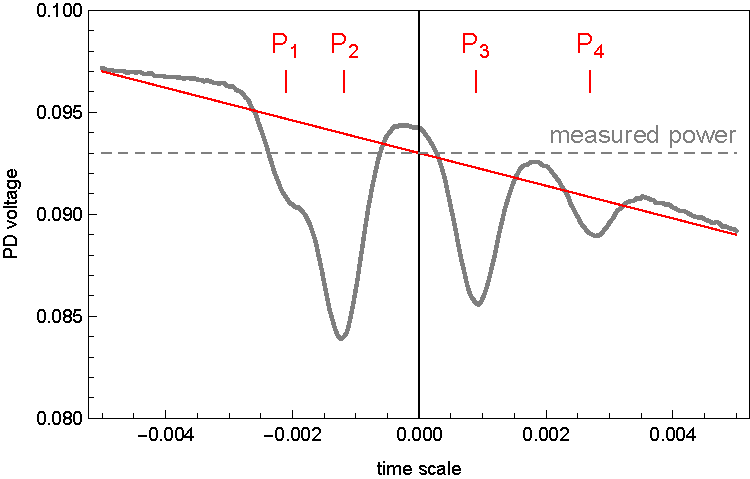
\includegraphics[width=.7\textwidth]{powercorrection}
    \caption{\label{fig:powercorrection} Linear approximation on power decrease}
\end{figure}

\begin{table}[h]
    \centering
    \begin{tabular*}{0.7\textwidth}{@{\extracolsep{\fill} }l c c}
    \toprule
    measured power: \SI{350}{\micro\watt} & & \\
    \midrule
    line & power [\si{\micro\watt}] & uncertainty [\si{\micro\watt}] \\
    \midrule
    \(^{87}\)Rb \(F=2\) & 355 & 21 \\
    \(^{85}\)Rb \(F=3\) & 353 & 21 \\
    \(^{85}\)Rb \(F=2\) & 347 & 20 \\
    \(^{87}\)Rb \(F=1\) & 343 & 20 \\
    \bottomrule
    \end{tabular*}
    \caption{\label{table:powercorrection} Power correction for \SI{350}{\micro\watt}
    measurement.}
\end{table}
\pagebreak
%********************************** % Third Section  **************************************
\section{Measured absorption coefficient} %Section - 4.3

To determine the absorption coefficient, we have to calculate the 
intensity for all transitions and measurements. For this we will use the 
estimated cross section of Section~\ref{sec:laser_dia_measurement} and the flat 
hat model \(I = \frac{power}{cross~section}\). The error bars are based on the
uncertainties of the power measurement given in Section~\ref{sec:absorption_spec}.
As an example the calculated intensities for the \SI{350}{\micro\watt} measurement 
can be found in Table~\ref{table:intcorrection}.

\bigskip
\begin{table}[h]
    \centering
    \begin{tabular*}{0.7\textwidth}{@{\extracolsep{\fill} }l c c}
    \toprule
    \multicolumn{3}{l}{calculated intensity at \SI{350}{\micro\watt}: \SI{168}{\watt\per\meter\squared}} \\
    \midrule
    line & intensity [\si{\watt\per\meter\squared}] & uncertainty [\si{\watt\per\meter\squared}] \\
    \midrule
    \(^{87}\)Rb \(F=2\) & 170 & 14 \\
    \(^{85}\)Rb \(F=3\) & 169 & 14 \\
    \(^{85}\)Rb \(F=2\) & 167 & 14 \\
    \(^{87}\)Rb \(F=1\) & 165 & 14 \\
    \bottomrule
    \end{tabular*}
    \caption{\label{table:intcorrection} Corresponding intensities to the power
    correction of the \SI{350}{\micro\watt} measurement.}
\end{table}

With Equation~\ref{eq:kappa_prime} and the length of the rubidium cell (\(L=\SI{0.1}{\meter}\))
one can now determine \(\kappa'_0\) for all lines and measurements.
As we can see in Fig.~\ref{fig:spectrumlegend} \(I_0\) corresponds to \(AmpM\)
and \(I(L,\nu_0)\) to \(AmpM-Amp\). It should be noted that we make an error on the 
assumption of \(AmpM~\widehat{=}~I_0 \), because of the linear decrease of 
amplitude/power over \(\nu \) (see Fig.~\ref{fig:powercorrection}).
We can limit the maximum error to \SI{3}{\percent}, due to the fact that the 
maximum relative amplitude deviation over the whole spectrum is on average \SI{6}{\percent}. 
This will be taken into account for the calculation of \(\kappa \). The uncertainties
for the different absorption coefficients are based on the uncertainties of the 
gaussian fit of the spectrum, which where extracted in Section~\ref{sec:modelfit}.
An example for the measured absorption coefficient is given in 
Table.~\ref{table:kappacorrection}.

\bigskip
\begin{table}[h]
    \centering
    \begin{tabular*}{0.7\textwidth}{@{\extracolsep{\fill} }l c c}
    \toprule
    \multicolumn{3}{l}{absorption coefficients at \SI{350}{\micro\watt} } \\
    \midrule
    line & \(\kappa \) [\si{\per\meter}] & uncertainty [\si{\per\meter}] \\
    \midrule
    \(^{87}\)Rb \(F=2\) & 0.38 & \num{0.17e-3} \\
    \(^{85}\)Rb \(F=3\) & 0.92 & \num{0.19e-3} \\
    \(^{85}\)Rb \(F=2\) & 0.62 & \num{0.20e-3} \\
    \(^{87}\)Rb \(F=1\) & 0.21 & \num{0.13e-3} \\
    \bottomrule
    \end{tabular*}
    \caption{\label{table:kappacorrection} Calculated absorption coefficients
    for \SI{350}{\micro\watt} measurement.}
\end{table}

The absorption coefficients calculated from our spectroscopy will then be fitted 
to the theoretical ones. 

%********************************** % Forth Section  **************************************
\section{Saturation intensity determination} %Section - 4.4

To account for isotope proportions and hyperfine level populations 
(see Sec.~\ref{sec:realrubidium}), each of the absorption coefficient models for 
our fit will be balanced, because it changes the atom density \(n_0\). In detail, we have a vapor constituted 
of the two atoms in two states each and their abundance depend on isotope 
concentration and on atom \(m_F\) level population. So we have
\begin{align}
    n_{0,tot} = n_{0,^{87}Rb~F=2} + n_{0,^{85}Rb~F=3} + n_{0,^{85}Rb~F=2} +
    n_{0,^{87}Rb~F=1}~.
\end{align} 
Where for each atom \(n_0\) is replaced by \(n_{0,tot} \times ratio_X \) 
(see Table.~\ref{table:kappamodelratio})

\bigskip
\begin{table}[h]
    \centering
    \begin{tabular*}{0.8\textwidth}{@{\extracolsep{\fill} }l c c c}
    \toprule
    \multicolumn{4}{l}{\(\kappa \) model adaptation} \\
    \midrule
    line & isotope abundance & hyperfine levels & \(ratio_X\) \\
    \midrule
    \(^{87}\)Rb \(F=2\) & 0.2784 & 5/8 & 0.174 \\
    \(^{85}\)Rb \(F=3\) & 0.7216 & 7/12 & 0.421\\
    \(^{85}\)Rb \(F=2\) & 0.7216 & 5/12 & 0.301\\
    \(^{87}\)Rb \(F=1\) & 0.2784 & 3/8 & 0.104 \\
    \midrule
    & & & 1.000 \\
    \bottomrule
    \end{tabular*}
    \caption{\label{table:kappamodelratio} Atomic density ratios of the different
    isotopes and hyperfine lines}
\end{table}

This leads to our model based on Equation~\ref{eq:kappa_final}

\begin{align}
    \kappa'_{0,X} = n_{0,tot} ~ratio_X ~ \frac{\pi^2 {\Gamma_\nu}^2}{I_{s}}~ h~\nu_0 ~ 
    \frac{c}{\nu_0} ~ \sqrt{ \frac{m_X}{2\pi~k_B T} } ~
    \frac{1}{\sqrt{1 + \frac{2I}{I_s}~\frac{\Gamma_\nu}{\Gamma_{\nu,tot}}}}~, 
\end{align}

where \(X\) stands for the different lines. The total atom density \(n_{0,tot} \) 
can be extracted out of the vapor-pressure model~\cite{vapour_pres}:
\begin{align}
    \log_{10} P_V = 4.312-\frac{4040}{T}~,
\end{align}
where \(P_V \) is the pressure in atmospheres and the ideal gas law, such that
\begin{align}
    n_{0,tot} = \frac{1}{k_B T}~10^{9.318-\frac{4040}{T}}~.
\end{align}

We use Mathematica to fit our data and because we want to include the obtained
error bars for the fit, we are restricted to a NonlinearModelFit. Moreover it is
only possible to have error bars on the y-axis of your data, which will be 
incorporated via a weight on every data point. For this reason we had to choose
the measurement with the larger error bars as our y-axis. We can see in our 
calculation that the error bars on \(\kappa \) are two orders of magnitude smaller 
than the errors bars on the calculated intensity 
(see Tables~\ref{table:intcorrection} and~\ref{table:kappacorrection}). However 
our models are \(\kappa \) depending on \(I \). For that reason we have to exchange
x- and y-axis of the used data sets and invert our model so we get \(I(\kappa)\) 
instead of \(\kappa(I)\).\\
To extract \(\kappa \) of our measurements we used the Beer-Lambert law, which 
assumes that \(\kappa \) is independent from \(I\). This assumption is only true
for intensities below \(I_{s}\). Therefore we have to limit our measurement data 
where the initial intensity is below \(I_{s} = \SI{126}{\watt\per\meter\squared}\), 
which is the theoretical one (see Fig.~\ref{fig:kappaplot}). Therefore we get 
following values and corresponding error bars for \(I_{s}\) and temperature 
\(T\) for every absorption line extracted (see Table~\ref{table:isat_temp}):

\bigskip
\begin{table}[h]
    \centering
    \begin{tabular*}{0.9\textwidth}{@{\extracolsep{\fill} }l c c c c}
    \toprule
    \multicolumn{5}{l}{saturation intensity and temperature} \\
    \midrule
    line & \(I_{s}\) [\si{\watt\per\meter\squared}] & uncertainty [\si{\watt\per\meter\squared}] &
           \(T \) [\si{\kelvin}] & uncertainty [\si{\kelvin}] \\
    \midrule
    \(^{87}\)Rb \(F=2\) & 45.6 & 1.8 & 336.9 & 0.4 \\
    \(^{85}\)Rb \(F=3\) & 51.7 & 2.5 & 338.2 & 0.5 \\
    \(^{85}\)Rb \(F=2\) & 37.2 & 2.6 & 334.5 & 0.6 \\
    \(^{87}\)Rb \(F=1\) & 30.7 & 3.3 & 332.3 & 0.9 \\
    \midrule
    mean value  & 41.3 & & 335.5 & \\
    \bottomrule
    \end{tabular*}
    \caption{\label{table:isat_temp} Fitted values of \(I_{s}\) and temperature.}
\end{table}

\begin{figure}[H]
    \centering
    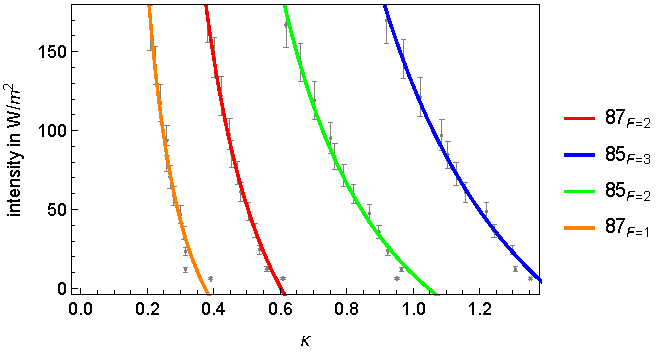
\includegraphics[width=.8\textwidth]{kappaplot}
    \caption{\label{fig:kappaplot} Plot of the four inverted absorption coefficients
    with corresponding error bars}
\end{figure}

